\documentclass[a4paper]{article}
\usepackage[spanish]{babel}
\usepackage[utf8]{inputenc}
\usepackage{graphicx}
\usepackage{enumerate}
\usepackage{listings}
\usepackage{color}
\usepackage{indentfirst}
\usepackage{fancyhdr}
\usepackage{latexsym}
\usepackage[colorlinks=true, linkcolor=black]{hyperref}
%\usepackage{makeidx}
%\usepackage{float}
\usepackage{calc}
\usepackage{amsmath, amsthm, amssymb}
\usepackage{amsfonts}
%\lstset{language=C}
\definecolor{gray}{gray}{0.5}
\definecolor{light-gray}{gray}{0.95}
\definecolor{orange}{rgb}{1,0.5,0}

\usepackage{fancyhdr}
\pagestyle{fancy}

%\renewcommand{\chaptermark}[1]{\markboth{#1}{}}
\renewcommand{\sectionmark}[1]{\markright{\thesection\ - #1}}

\fancyhf{}

\fancyhead[LO]{Sección \rightmark} % \thesection\ 
\fancyfoot[LO]{\small{Carolina Lang, Laura Muiño, Martín Ventura}}
\fancyfoot[RO]{\thepage}
\renewcommand{\headrulewidth}{0.5pt}
\renewcommand{\footrulewidth}{0.5pt}
\setlength{\hoffset}{-0.8in}
\setlength{\textwidth}{16cm}
%\setlength{\hoffset}{-1.1cm}
%\setlength{\textwidth}{16cm}
\setlength{\headsep}{0.5cm}
\setlength{\textheight}{25cm}
\setlength{\voffset}{-0.7in}
\setlength{\headwidth}{\textwidth}
\setlength{\headheight}{13.1pt}

\renewcommand{\baselinestretch}{1.1}  % line spacing


% \setcounter{secnumdepth}{2}
\usepackage{underscore}
\usepackage{caratula}
\usepackage{url}
\usepackage{float}

\newcommand{\cod}[1]{{\tt #1}}
\newcommand{\negro}[1]{{\bf #1}}
\newcommand{\ital}[1]{{\em #1}}
\newcommand{\may}[1]{{\sc #1}}
\newcommand{\tab}{\hspace*{2em}}

\hypersetup{
 pdfstartview= {FitH \hypercalcbp{\paperheight-\topmargin-1in-\headheight}},
 pdfauthor={Grupo},
 pdfsubject={Dise\~{n}o}
}

\lstdefinestyle{customc}{
  backgroundcolor=\color{light-gray},
  belowcaptionskip=1\baselineskip,
  breaklines=true,
  numbers=left,
  xleftmargin=\parindent,
  language=C,
  showstringspaces=false,
  basicstyle=\footnotesize\ttfamily,
  keywordstyle=\bfseries\color{blue},
  commentstyle=\itshape\color{gray},
  identifierstyle=\color{black},
  stringstyle=\color{orange},
}

\lstdefinestyle{customasm}{
  backgroundcolor=\color{light-gray},
  belowcaptionskip=1\baselineskip,
  numbers=left,
  xleftmargin=\parindent,
  language=[x86masm]Assembler,
  keywordstyle=\bfseries\color{blue},
  basicstyle=\footnotesize\ttfamily,
  commentstyle=\itshape\color{gray},
}

\lstset{escapechar=@}


\begin{document}

\thispagestyle{empty}
\materia{Sistemas Operativos}
\submateria{Primer Cuatrimestre de 2015}
\titulo{Trabajo Práctico I}
\subtitulo{Scheduling}
\integrante{Carolina Lang}{906/12}{carolinalang93@gmail.com}
\integrante{Laura Muiño}{399/11}{mmuino@dc.uba.ar}
\integrante{Alejandro Martín Ventura}{249/11}{vn2.amv@gmail.com}

\makeatletter

\maketitle
\newpage

\thispagestyle{empty}
\vfill

\thispagestyle{empty}
\vspace{3cm}
\tableofcontents
\newpage

\newenvironment{myindentpar}[1]
{\begin{list}{1}
         {\setlength{\leftmargin}{#1}}
         \item[]
}
{\end{list} }

%\normalsize
\newpage

% -------------------------------------------------------
% Introducccion
% -------------------------------------------------------
\section{Introducción}


El scheduling es un método mediante el cual se le da a las tareas de un computador acceso a lo recursos del mismo. Se busca que un scheduler cumpla diversos requisitos, como ser justo en cuanto a los recursos que se le asigna a cada proceso, conseguir terminar una gran cantidad de procesos en poco tiempo, etc.
En este trabajo se estudiaran distintos schedulers sobre distintos lotes de tareas y el efecto que distintas características  tienen sobre el desempeño de cada uno, por ejemplo quantum, cantidad de cores, tiempo de migración, de cambio de contexto,  cantidad de tareas etc. Para esto se utilizará un simulador que dadas las implementaciones de estos schedulers nos permite obtener información sobre como se comportan con un lote de tareas dado. 
% -------------------------------------------------------
% Ejercicios 1 y 2
% -------------------------------------------------------
\section{Ejercicios 1 y 2}
Para ver gráficamente el comportamiento del scheduler FCFS, creamos un lote de tareas que tenía uso intensivo de CPU, y dos tareas que sólo ejecutan llamadas bloqueantes (una con muchas llamadas cortas y una con pocas más largas).
\begin{figure}[h]
  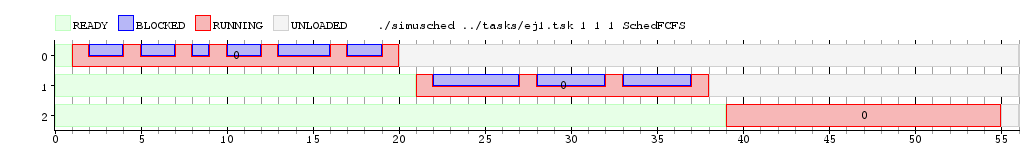
\includegraphics[width=\textwidth]{ej1-2/figs/ej1-1core.png}
  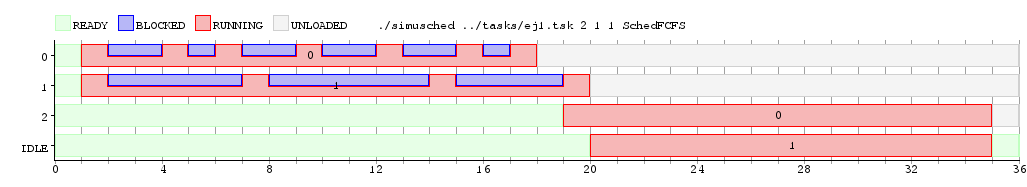
\includegraphics[width=\textwidth]{ej1-2/figs/ej1-2core.png}
  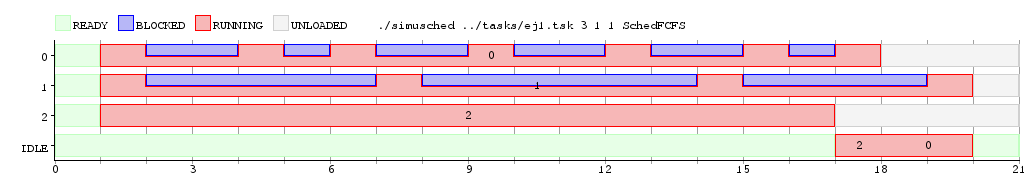
\includegraphics[width=\textwidth]{ej1-2/figs/ej1-3core.png}
  \caption{Diagramas de Gantt para la simulación con 1, 2 y 3 núcleos respectivamente.}
\end{figure}

Los procesos se ejecutan siempre hasta que se terminan, por lo tanto permanecen ejecutando aún estando bloqueados.

% -------------------------------------------------------
% Ejercicios 3 y 4
% -------------------------------------------------------
\newpage
\section{Ejercicios 3 y 4 (Round Robin)}
Para testear el algoritmo de Round Robin que permite migración utilizamos los siguientes lotes de tareas:

\textbf{Primer lote:}

\begin{lstlisting}
 # Lote solo con tareas que consumen CPU
 *4 TaskCPU 6
\end{lstlisting}

Sobre el primer lote de tareas hicimos gráficos variando el \textit{quantum} (para 1 y 2 ciclos).
\begin{figure}[h]
 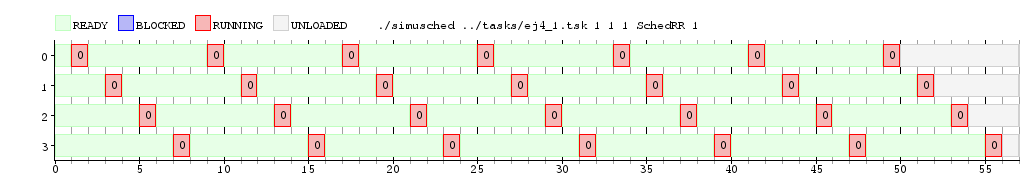
\includegraphics[width=\textwidth]{ej3-4/figs/lote1-quantum1.png}
 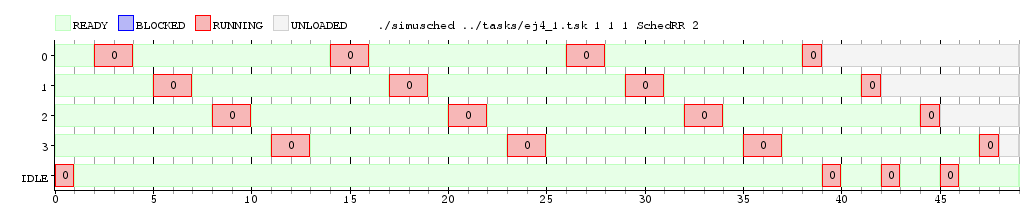
\includegraphics[width=\textwidth]{ej3-4/figs/lote1-quantum2.png}
 \caption{Diagramas de Gantt sobre el primer lote de tareas (para un núcleo, y con quantum igual a 1 y 2, respectivamente).}
 \label{fig:ej4:quantum}
\end{figure}

En la figura~\ref{fig:ej4:quantum} vemos que el algoritmo de Round Robin ejecuta las tareas secuencialmente durante un quantum (que varía de longitud según el caso).

Vemos que sube el tiempo en el que el procesador ejecuta cambios de contexto, porque no se ejecuta una tarea de principio a fin como en el caso anterior.
Al mismo tiempo, mientras más largo es el quantum, menos tiempo se pierde en dichos cambios de contexto (el tiempo de ejecución baja de 56 a 48, incluso con un costo bajo de cambio de contexto).

\textbf{Segundo lote:}
El segundo lote contiene también tareas con bloqueos.

\begin{lstlisting}
 # Tareas que se bloquean y que comen CPU
 *2 TaskConsola 5 1 10
 @3
 *2 TaskCPU 15
\end{lstlisting}

En estos casos el algoritmo de Round Robin tiene la ventaja adicional de que (como vemos en la figura~\ref{fig:ej4:cores}), ante un bloqueo, el procesador cambia de proceso y aprovecha el tiempo de CPU.
\begin{figure}[h]
 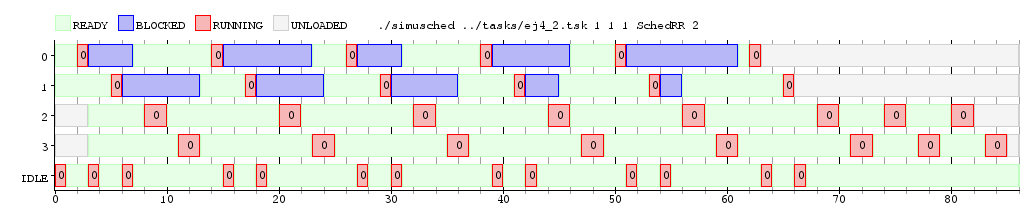
\includegraphics[width=\textwidth]{ej3-4/figs/lote2-1core.png}
 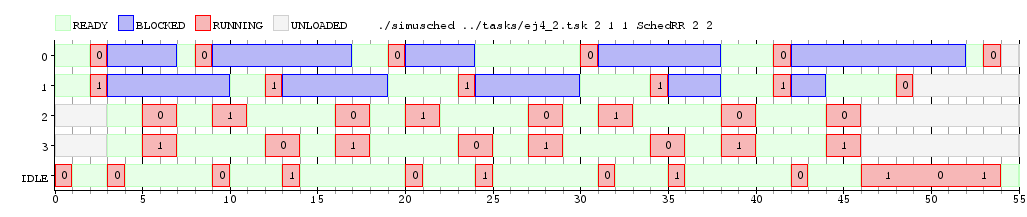
\includegraphics[width=\textwidth]{ej3-4/figs/lote2-2core.png}
 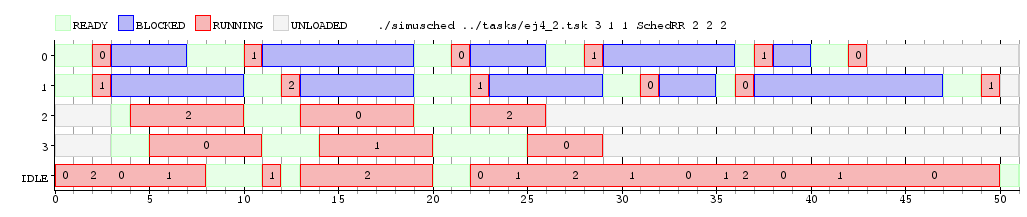
\includegraphics[width=\textwidth]{ej3-4/figs/lote2-3core.png}
 \caption{Diagramas de Gantt sobre el segundo lote de tareas (para 1, 2 y 3 núcleos, fijando el quantum en 2).}
 \label{fig:ej4:cores}
\end{figure}

En el caso de un núcleo no se nota tanto la mejora porque todos los bloqueos terminan antes de que el ciclo vuelva al mismo proceso, pero ya en 2 núcleos vemos que el algoritmo, en el tick 9, asigna la tarea 2 (en vez de la 1) al procesador 1, porque el otro no estaba disponible.
Este comportamiento se repite a lo largo del resto de la ejecución. En el caso de 3 núcleos, incluso, el mismo proceso puede ejecutar durante varios quantums seguidos a pesar de que sean más la cantidad de tareas que la de procesadores.



% -------------------------------------------------------
% Ejercicio 5
% -------------------------------------------------------
\newpage
\section{Ejercicio 5}


a) Los autores intentan resolver el problema de diseñar un  scheduler para un computador que desarrolla tareas periódicas de monitoreo y control de procesos, en un marco en el cual debe ser garantizada la ejecución en tiempo real.  Es decir, en un sistema que cumple $n$ tareas de monitoreo/control, donde cada una de ellas se ejecuta cada cierto tiempo $T_i$, y tiene una duración de $C_i$ el scheduler debe ser capaz de , para cada tarea $t_i$, ejecutarla antes de que llegue a su deadline(tiempo entre dos request de una misma tarea). Este objetivo estudia en el marco de las siguientes restricciones.
\begin{itemize} 
\item Los requests para las tareas que tienen deadline estrictos son periodicos a intervalos constantes.  
\item Los deadlines consisten en que la ejecucion de una tarea debe terminar antes de que se produzca el siguiente request para esta.
\item Las tareas son independientes entre si.
\item Los run-time's de cada tarea son constantes (sin contar interrupciones)
\item Las tareas no periodicas en el sistema son especiales. Son tareas de incialización o manejo de errores, no tienen deadlines estrictos, y desplazan a las tareas periodicas en el tiempo mientras ellas estan corriendo.
\end{itemize} 
Asumiendo estos puntos es posible deducir y demostrar resultados analíticos acerca de los posibles métodos de scheduling que puedan cumplir los requerimientos mencionados.

b) En el caso del algoritmo basado en prioridades fijas, el mínimo de los factores de utilización del procesador para todos los conjuntos de tareas es de 70%. Además, si bien el algoritmo es óptimo, lo es solo en el sentido en que si otro algoritmo estático puede realizar con éxito el scheduling de un conjunto de tareas, el primero también puede, pero esto no dice nada del caso mas general en que el algoritmo es dinámico, lo cual incluye al caso estatico porque puede haber casos donde la mejor asignación dinamica, de un resultado estatico. Esto motiva a buscar un algoritmo más general e inteligente que pueda incrementar ese valor, y posiblemente aumentar la cantidad de conjuntos de tareas para los cuales el algoritmo es factible.


c) El teorema 7 nos dice que el scheduler es factible si se cumple la condición:

$\frac{C_1}{ T_1} + \frac{C_2}{ T_2} + \frac{C_3}{ T_3} + ... + \frac{C_n}{ T_n}  \leq 1$

Siendo $C_i$ el run-time de la tarea y $T_i$ los periodos de requerimientos. Esta restricción implica que los tiempos de run-time no pueden ser cercanos a los periodos de requerimiento, ya que si es así dejaria poco margen a las otras tareas para ejecutarse. Por ejemplo, podemos imaginar el caso en que una tarea tiene un run-time igual a su request period, en ese caso la tarea necesitaria todo el tiempo de procesador para ella, no pudiendo nunca asignar las otras tareas.  Si los run-times sin embargo, son notablemente mas pequeños que los request periods, queda mucho tiempo entre la llamada a una tarea y su llamada subsiguiente, pudiendo utilizarse ese tiempo para correr otros procesos.



% -------------------------------------------------------
% Ejercicio 6
% -------------------------------------------------------
% No hay nada de informe que hacer sobre este ejercicio

% -------------------------------------------------------
% Ejercicio 7
% -------------------------------------------------------
\section{Ejercicio 7}

Bajo la métrica tiempo de respuesta (esto es, el tiempo que tarda desde que se genera un pedido hasta que se obtiene la respuesta) esperamos que el quantum óptimo sea el menor posible, ya que a esta métrica solo concierne la cantidad de tiempo que pasa desde el pedido hasta la atención de la tarea, y con un quantum mayor, se es`era que cada tarea deba esperar mas tiempo hasta ser atendida, ya que debe esperar a que las tareas que están corriendo terminen su quantum. 


Sin embargo, al tener un quantum mas grande, se pierde menos tiempo realizando cambios de contexto, siguiendo este razonamiento, un quantum alto debería tener un mejor puntare en una medida que tenga que ver con la velocidad de ejecución de las tareas.

Es así que proponemos como segunda medida el THROUGHPUT (cantidad de procesos que terminan por unidad de tiempo). En este caso se espera como se comento anteriormente un desempeño superior de un quantum mas alto.


Presentamos 4 instancias de cuatro tareas TaskBatch con 3 bloqueos para todas las tareas. Los gráficos resultantes son los siguientes y los usamos como base para las conclusiones más abajo.


\begin{figure}[H]
  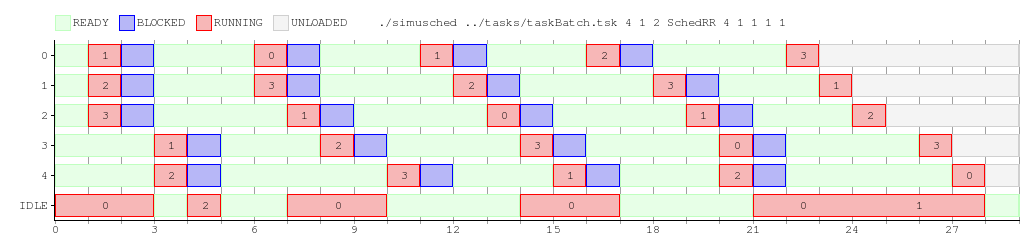
\includegraphics[width=\textwidth]{ej7/salida.png}
  \caption{Tarea con 1 quantum.}
\end{figure}

\begin{figure}[H]
  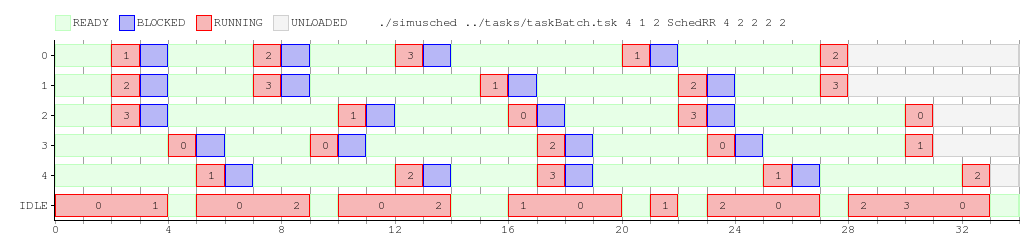
\includegraphics[width=\textwidth]{ej7/salida2.png}
  \caption{Tarea con 2 quantums.}
\end{figure}

\begin{figure}[H]
  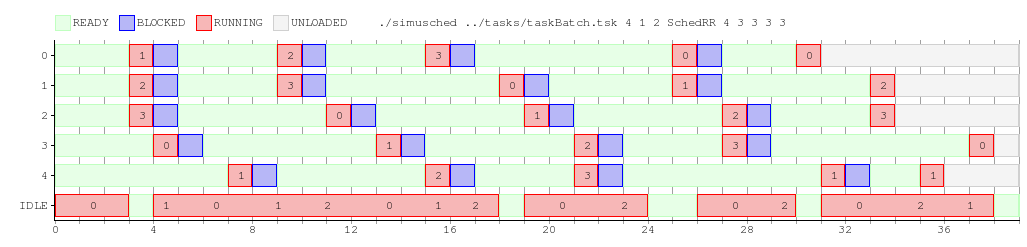
\includegraphics[width=\textwidth]{ej7/salida3.png}
  \caption{Tarea con 3 quantums.}
\end{figure}

\begin{figure}[H]
  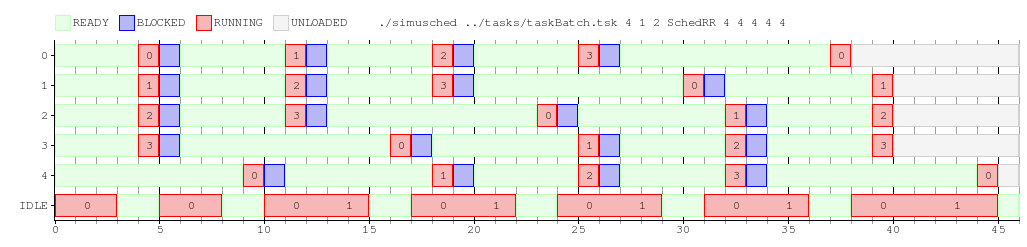
\includegraphics[width=\textwidth]{ej7/salida4.png}
  \caption{Tarea con 3 quantums.}
\end{figure}


Como se puede observar en la experimentación realizada el quantum mas chico fue el que mejor resultados dio en cuanto al tiempo de respuesta.


% -------------------------------------------------------
% Ejercicio 8
% -------------------------------------------------------
\newpage

\section{Ejercicio 8 (Migración vs. No Migración)}
Con el objetivo de comparar el scheduling round robin con y sin migracion de nucleos, se realizaron distintas experimentaciones con distintos costos de cambio de contexto, de migración de núcleo, cantidad de núcleos, el quantum de cada uno y duración de quantum para cada cpu.

Con el objetivo de simplificar la experimentción algunos parámetros se dejaron fijos, estos fueron elejidos porque no producen un efecto sobre el resultado al variar, teniendo o no teniendo migración activada. En particular los parámetros que se dejaron fijos en este caso fueron el costo de context switch, que no afecta el resultado ya que con o sin migración se realizan la misma cantidad de context switch's.

Primero se muestran los resultados para tiempo de migración = 1, dos nucleos, para 4 tareas.
\begin{figure}[h]
  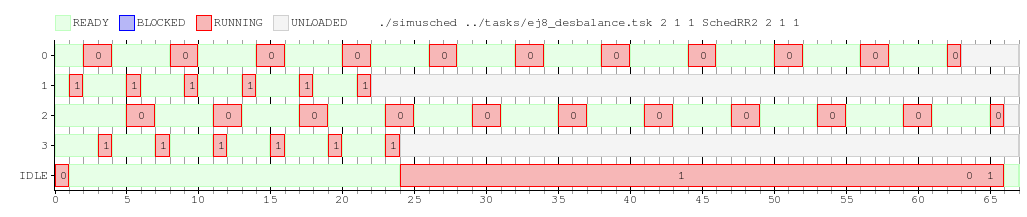
\includegraphics[width=\textwidth]{ej8/figs/sinMigracion.jpg}
  \caption{Diagramas de Gantt sin migración.}
\end{figure}


\begin{figure}[h]
  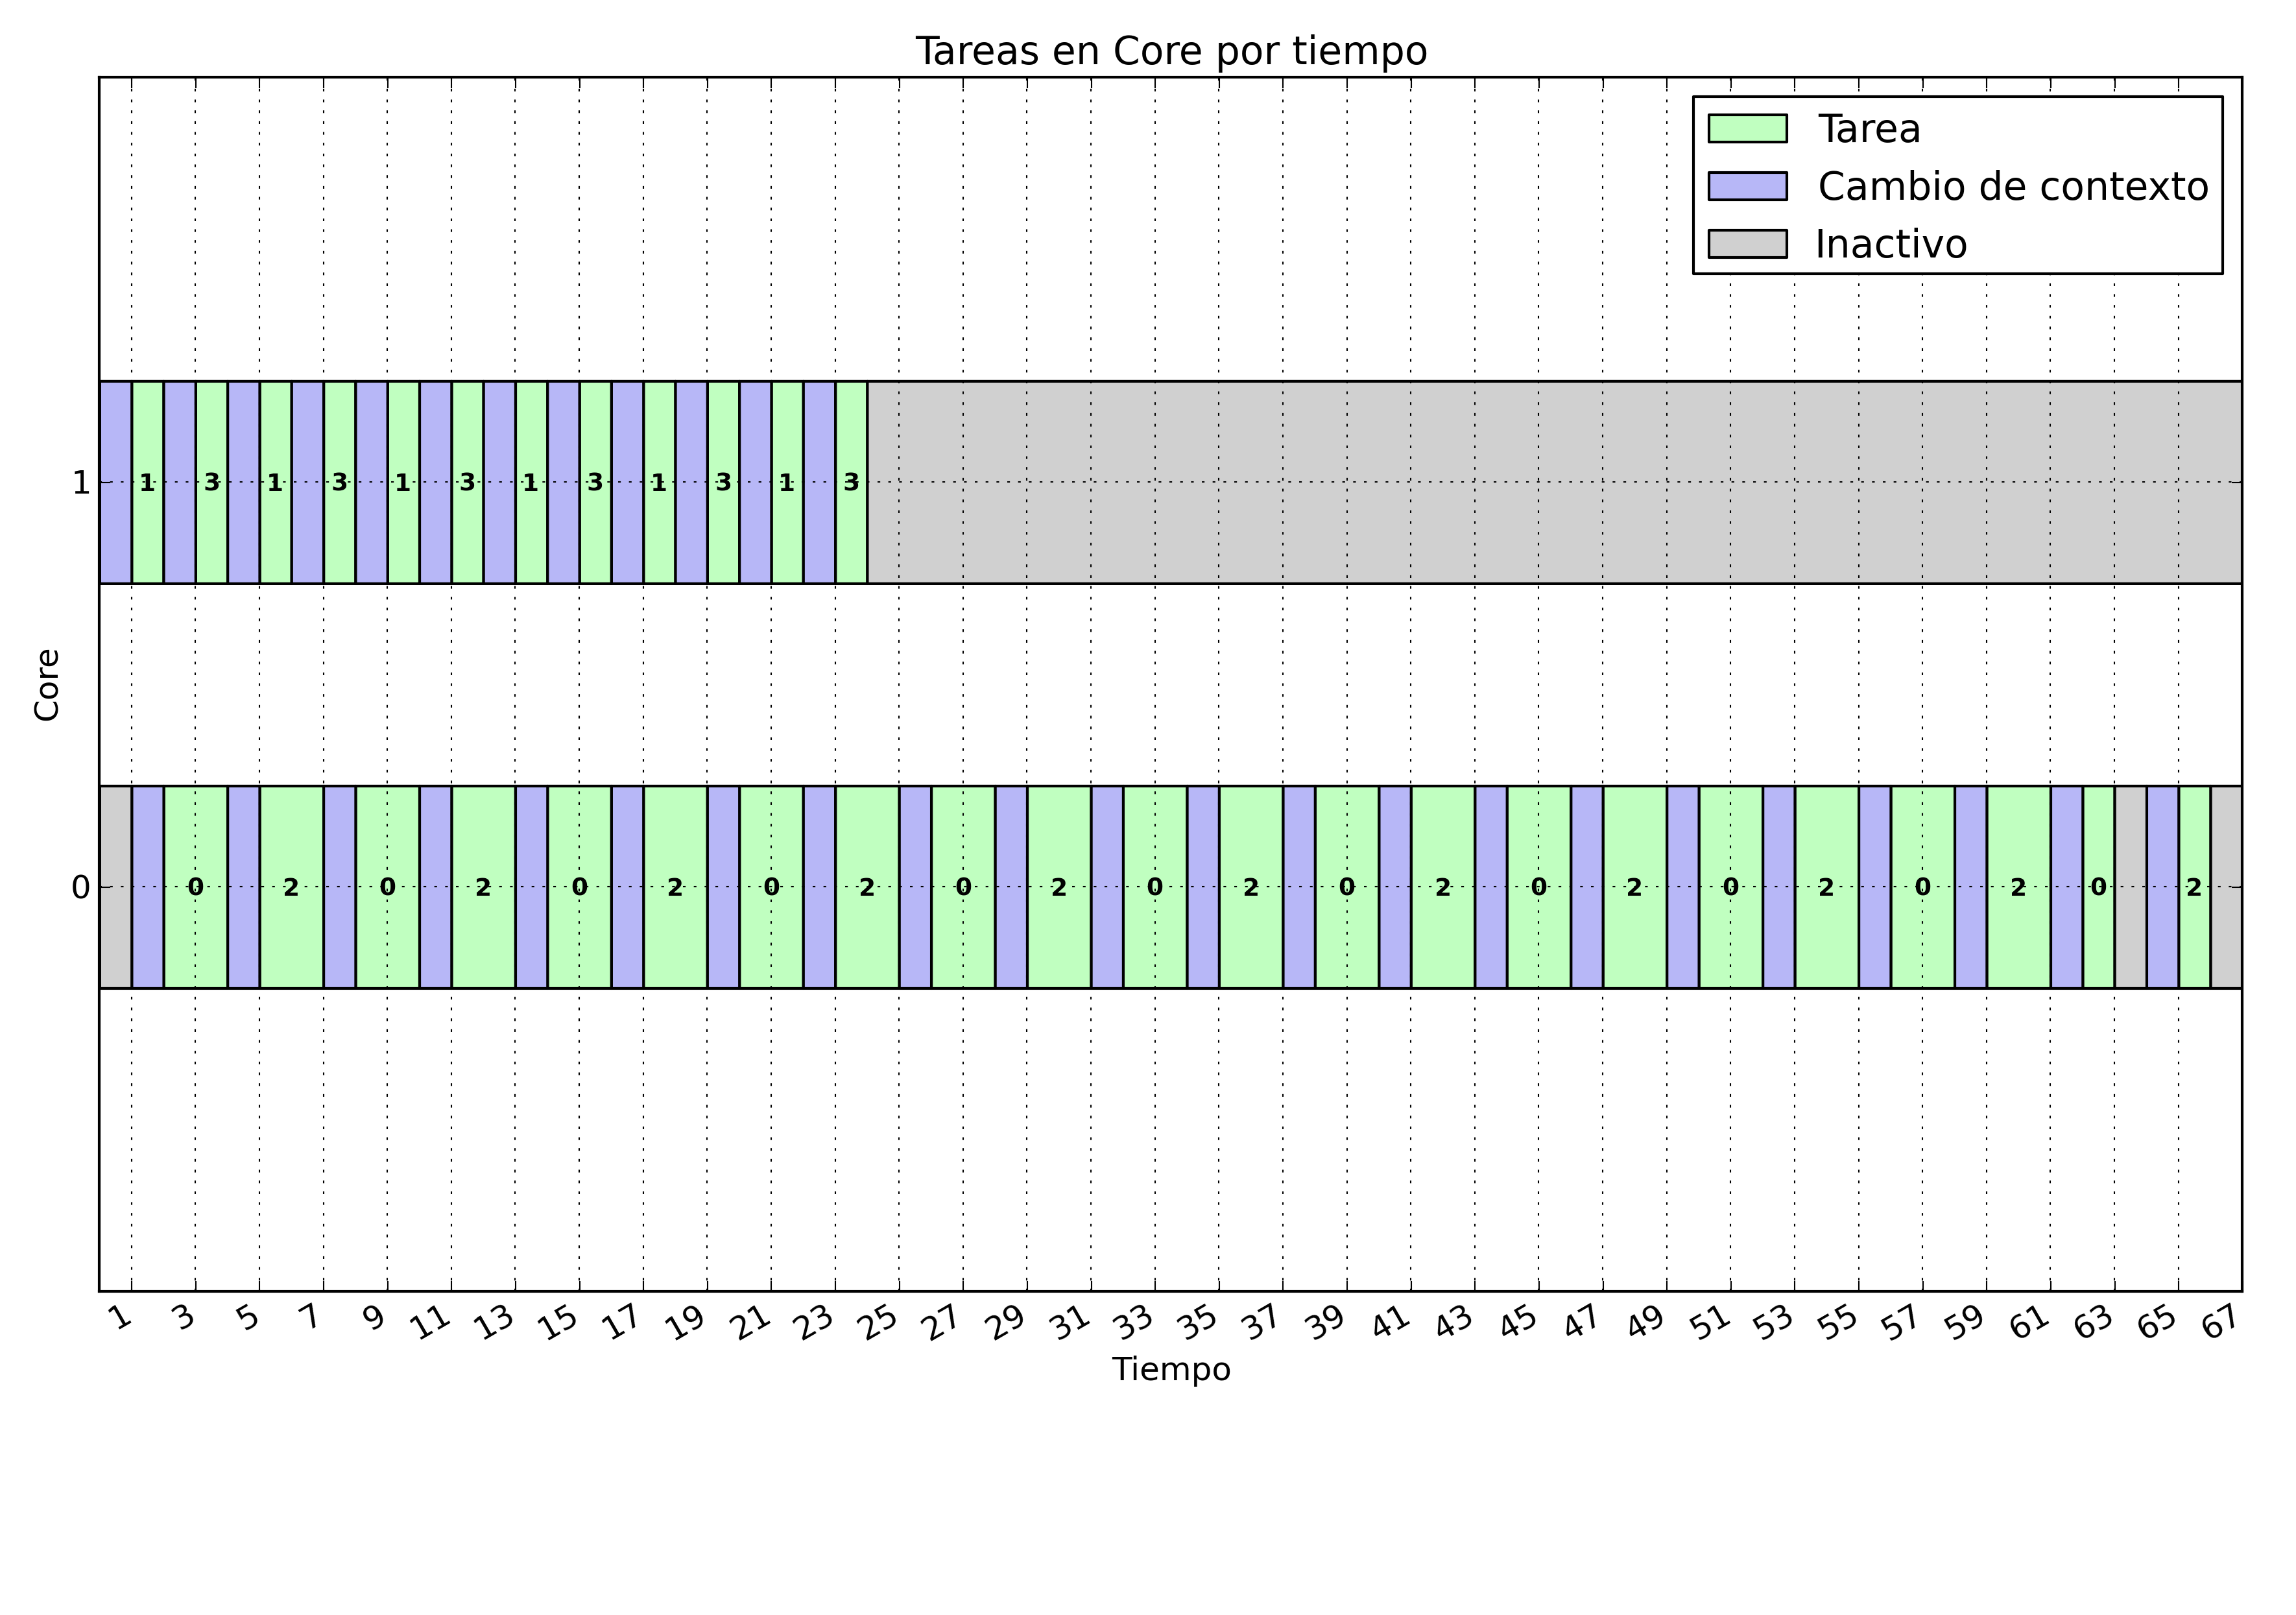
\includegraphics[width=\textwidth]{ej8/figs/coresSinMigracion.png}
  \caption{Diagramas de procesadores sin migración.}
\end{figure}


\begin{figure}[h]
  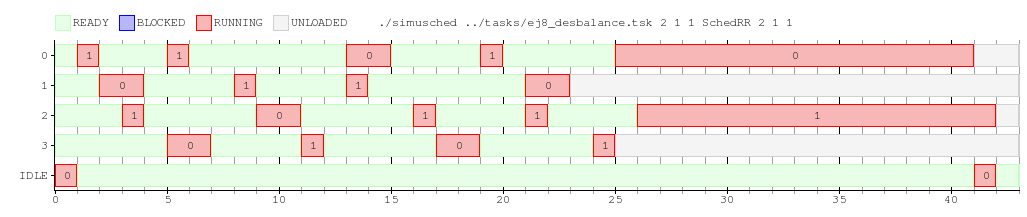
\includegraphics[width=\textwidth]{ej8/figs/conMigracion.jpg}
  \caption{Diagramas de Gantt con migración.}
\end{figure}


\begin{figure}[h]
  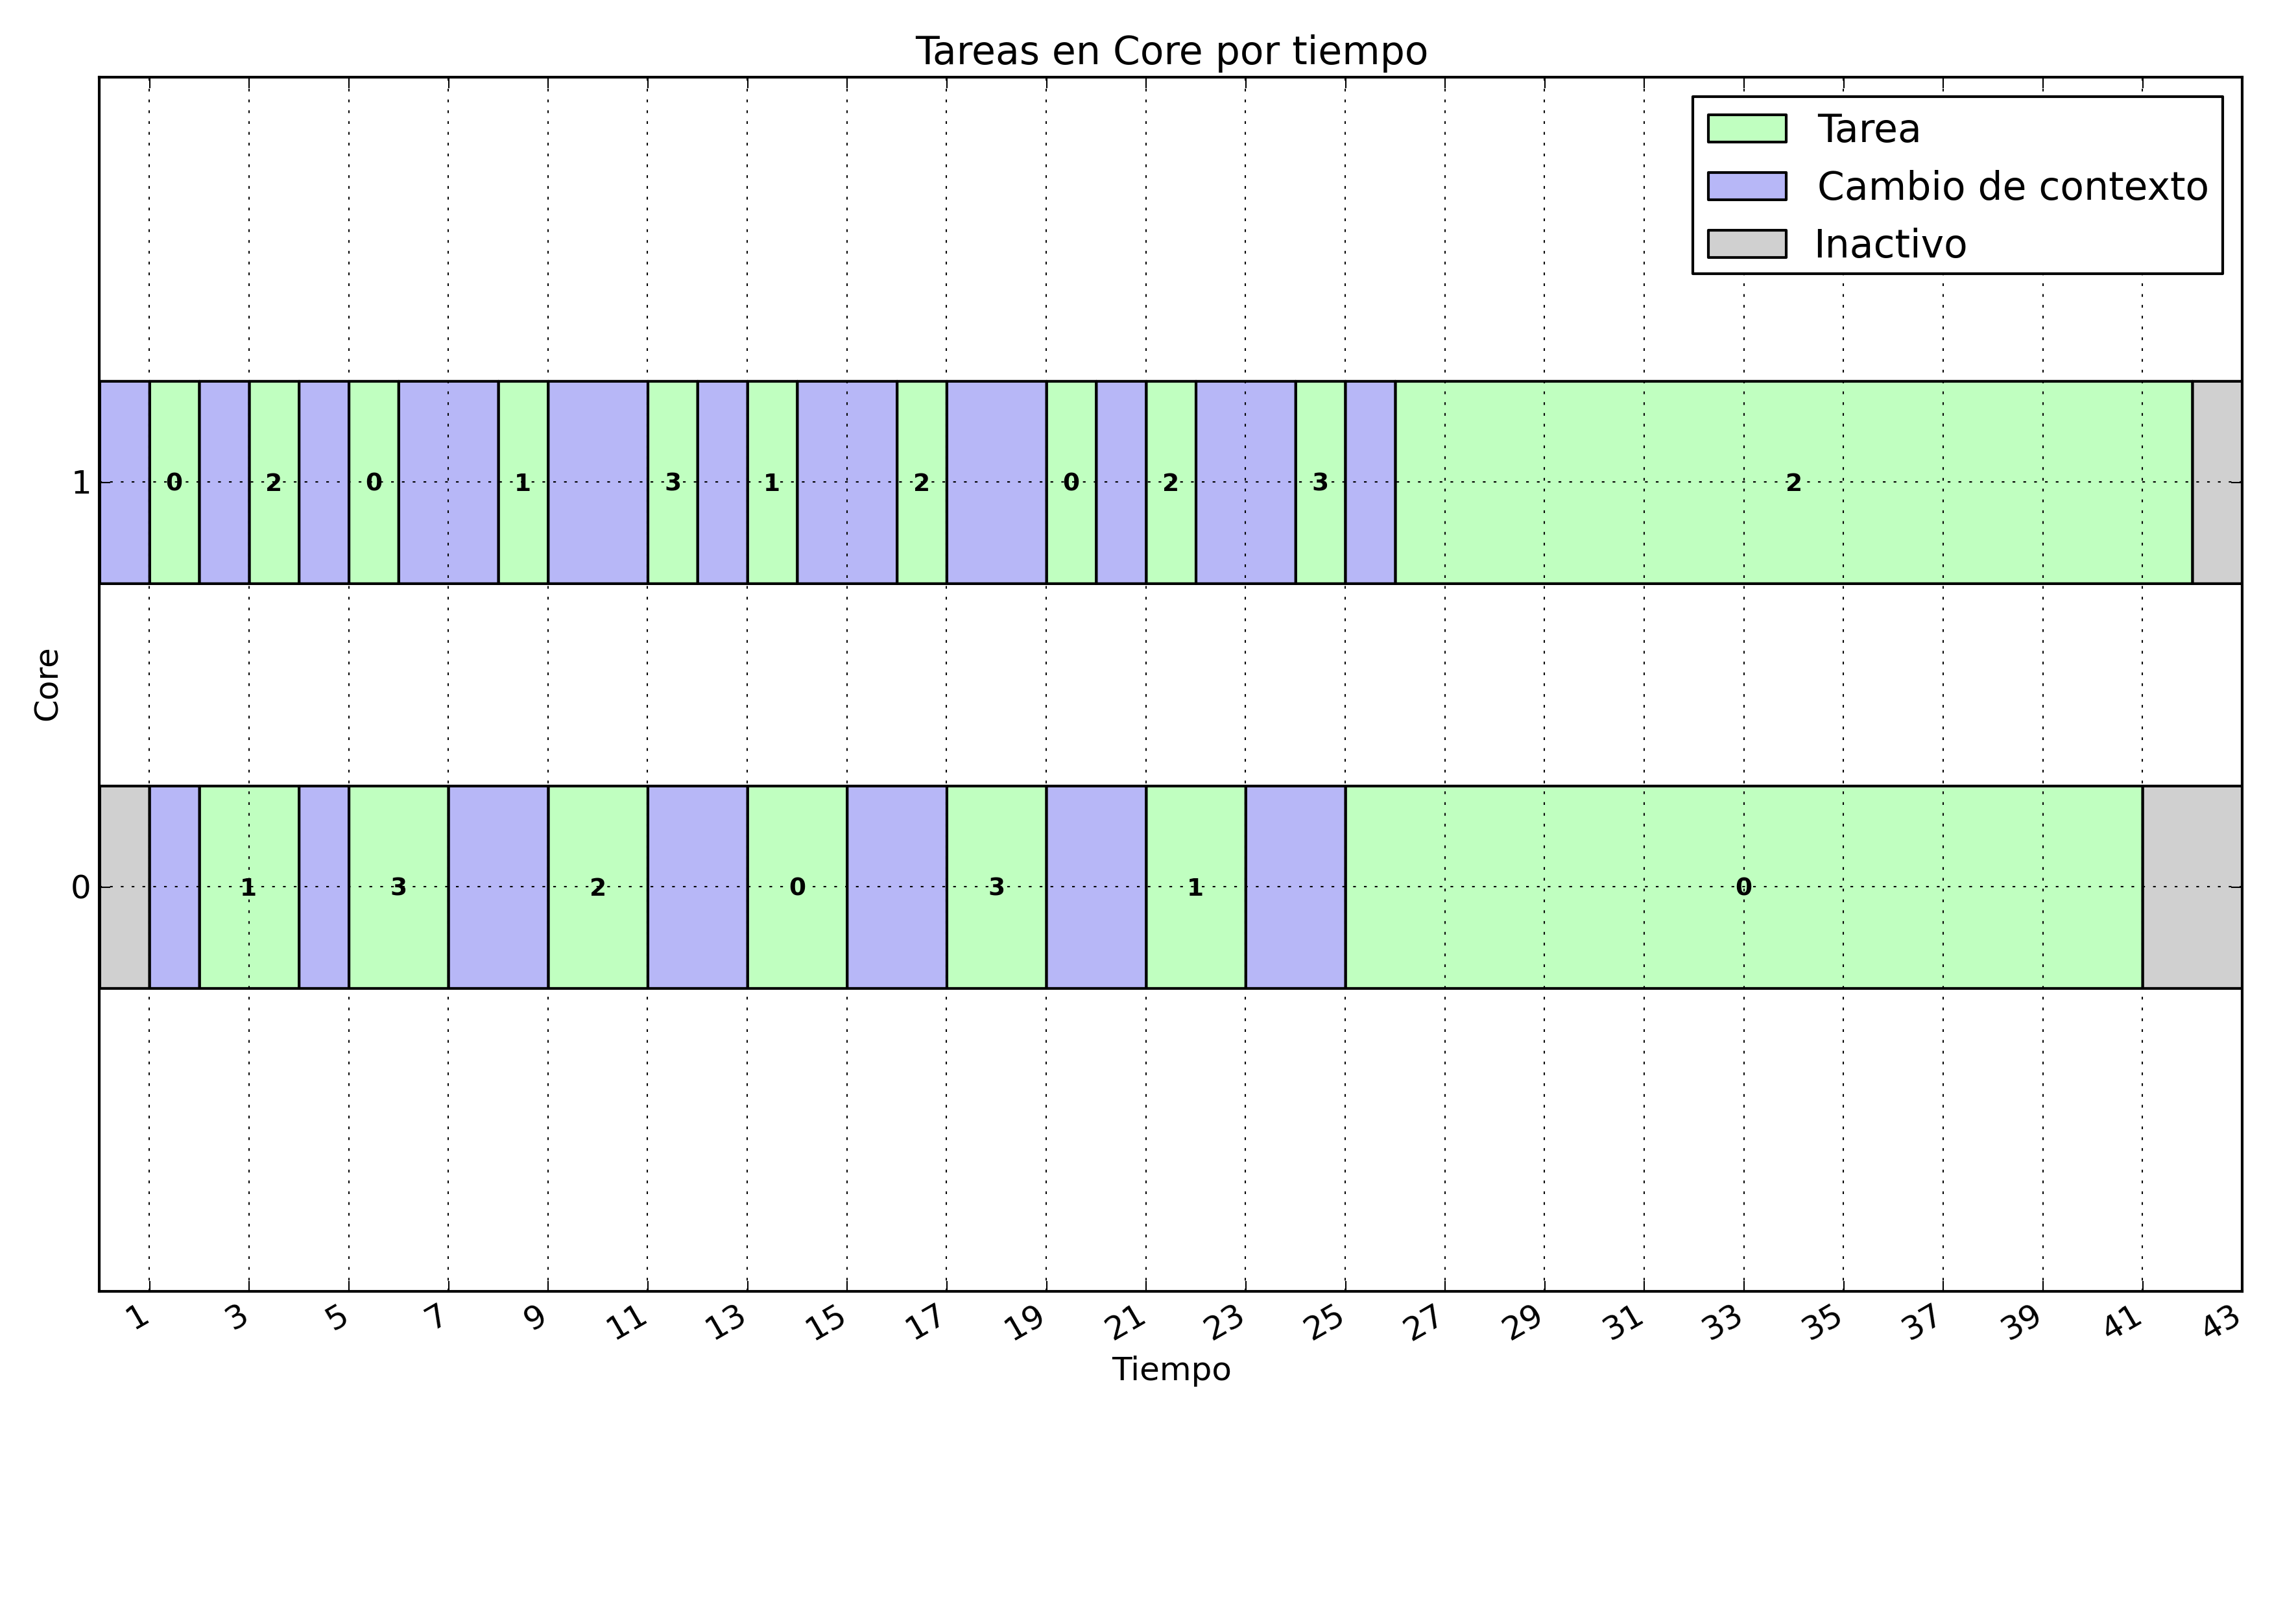
\includegraphics[width=\textwidth]{ej8/figs/coresConMigracion.png}
  \caption{Diagramas de procesadores con migración.}
\end{figure}

Como puede observarse mediante la activación de la migración se redujo el tiempo total de ejecución de 66 a 42 ticks.

Se consiguieron posteriormente resultados para distintas cantidades de tareas y nucleos. En todos los casos se obtuvo un resultado similar. En general, las corridas con migración mostraron un mayor tiempo de ejecución que las corridas sin migración. Se observó que en el caso de las corridas con migración se realizaban muchas migraciones que no daba utilidad alguna, y que consumían tiempo. En el caso en que no habia migraciones, se notaba que llegando al final de la ejecucion, uno o varios nucleos permanecian inactivos, mientras que otros trabajaban en varias tareas. Si bien esto no es óptimo porque hay procesadores ociosos a los que  podrían migrarse tareas, en base a nuestros resultados podemos concluir que en el caso general el beneficio de no gastar tiempo migrando suele superar este problema.

Se condujeron también experimentaciones variando los quantums de los núcleos. Se espera que en el caso de las migraciones, el tener quantums más grandes aporte beneficios extra comparando con el caso no migrante, ya que solo unas pocas migraciones son necesarias, al momento de tener procesadores ociosos, y tener muchas migraciones antes de eso alarga la ejecución.

\begin{figure}[H]
  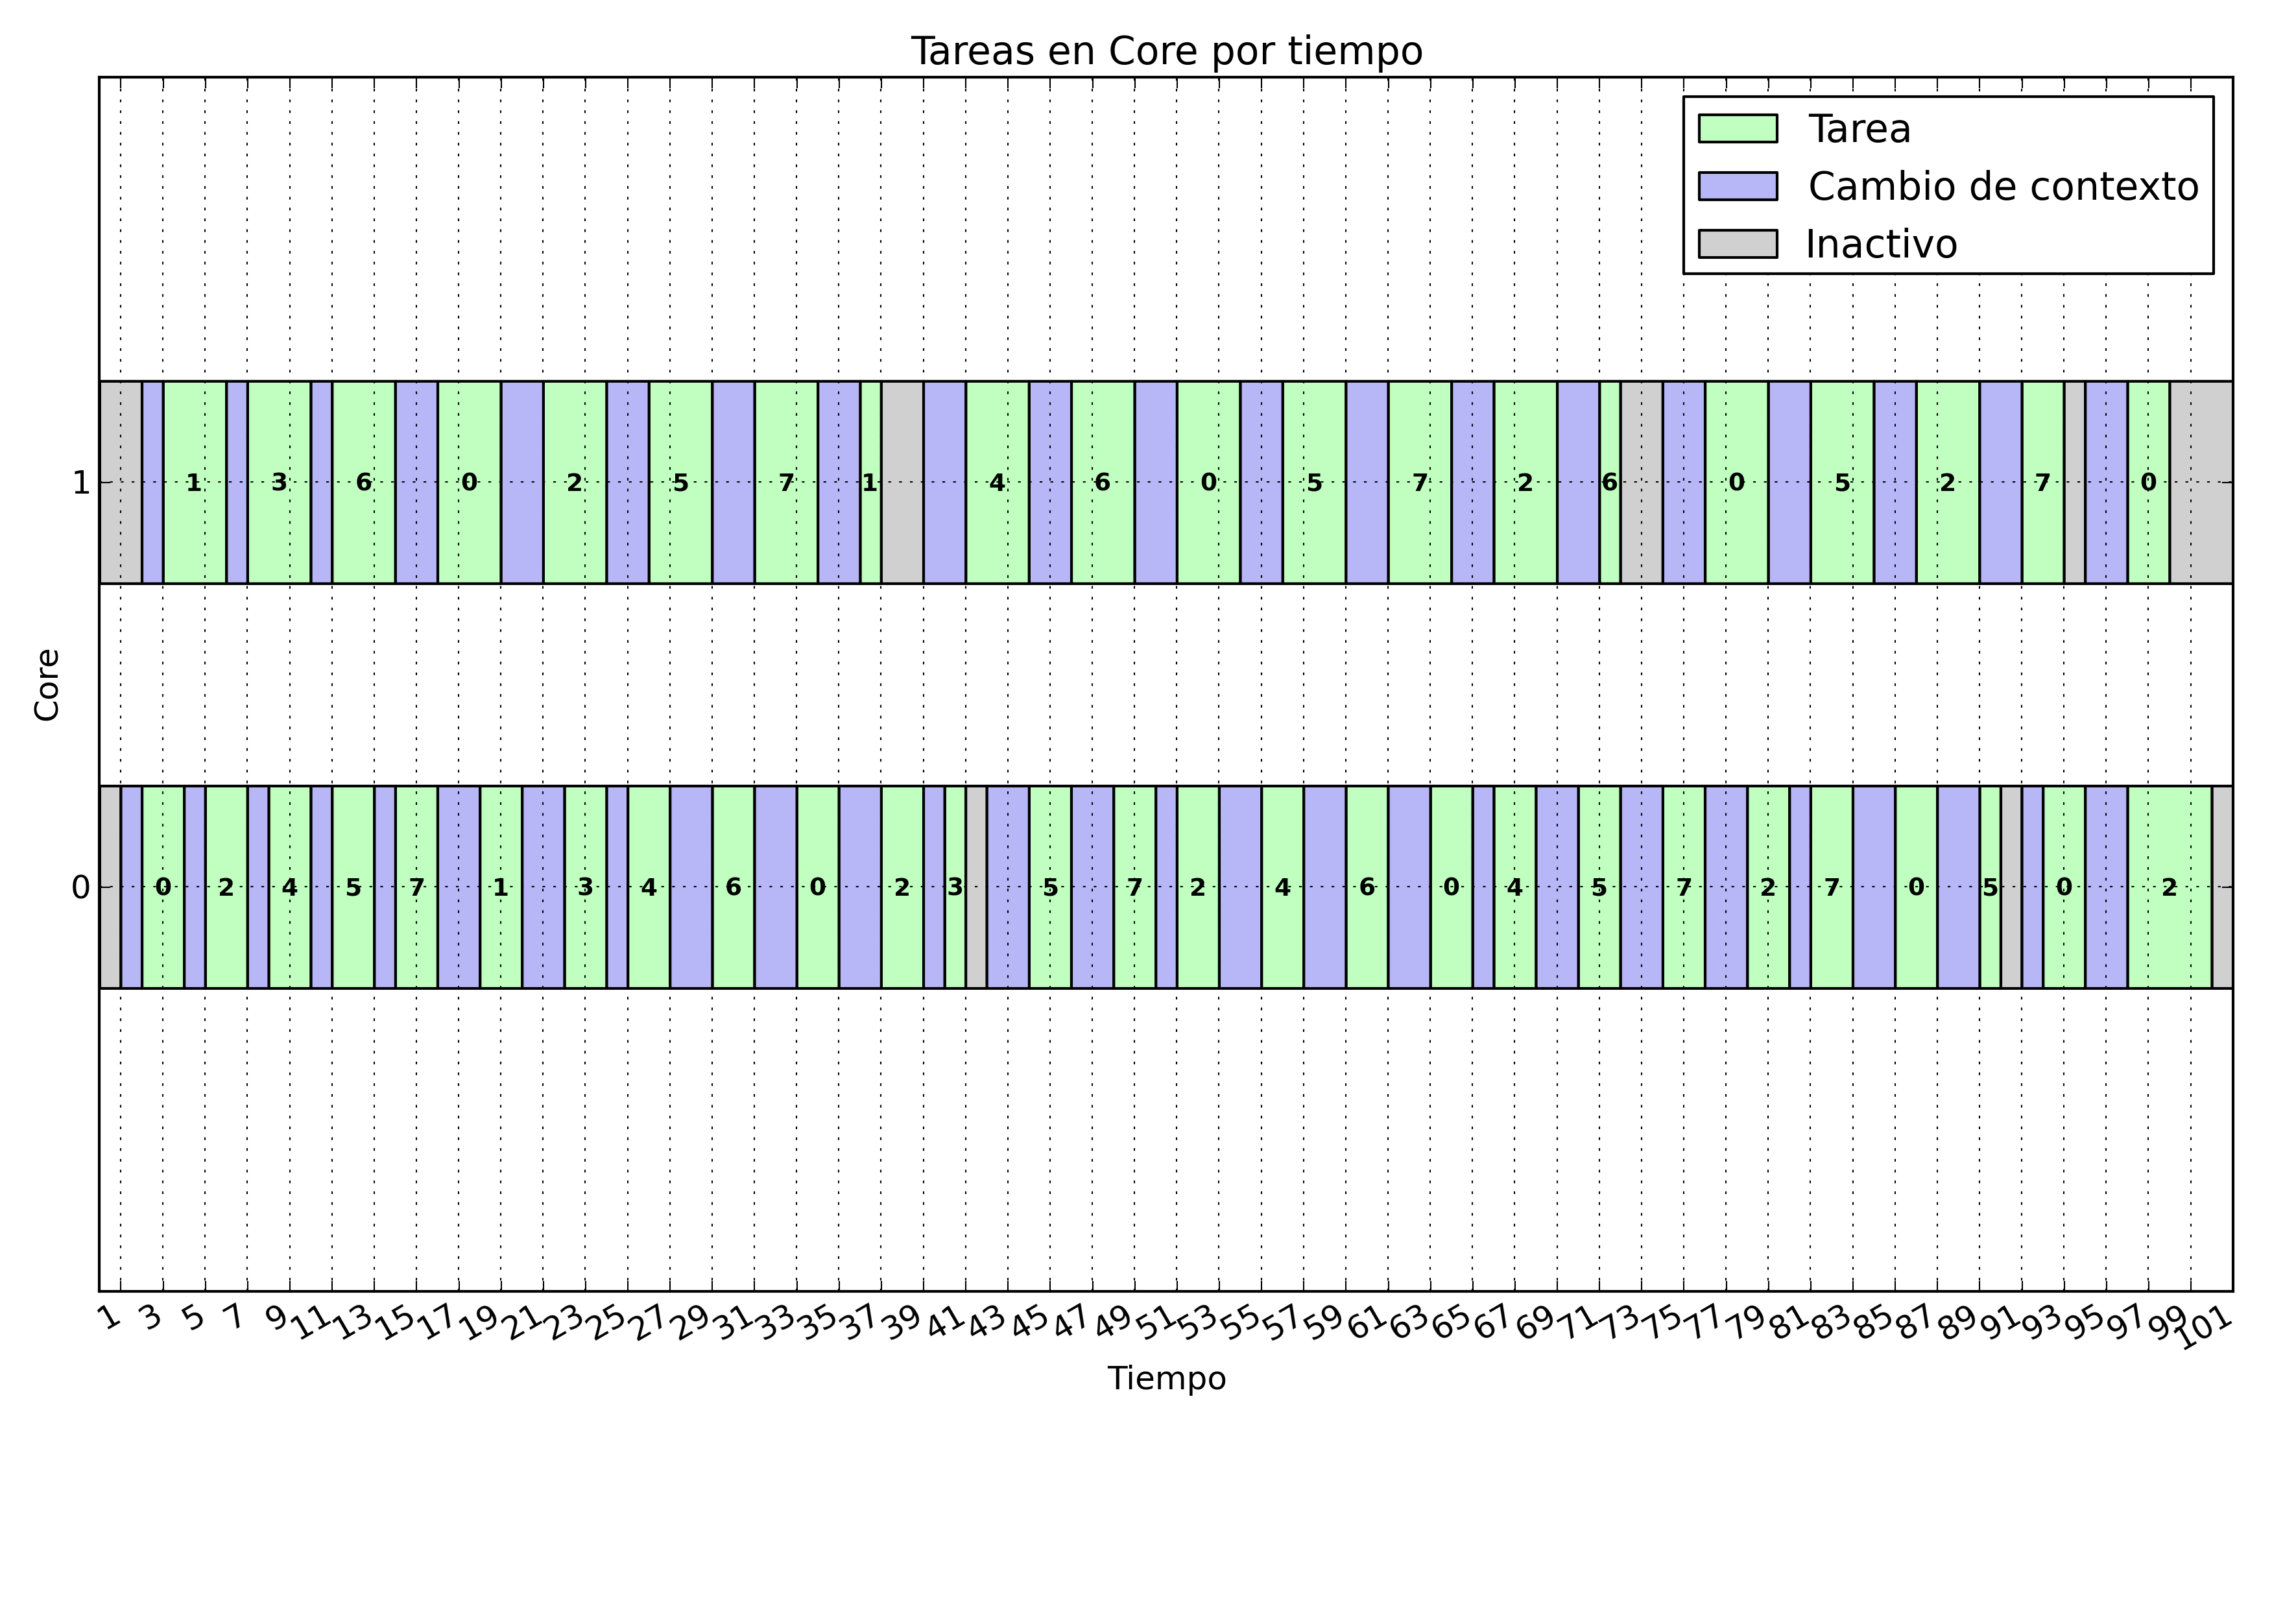
\includegraphics[width=\textwidth]{ej8/figs/C2Q3conMigracion.png}
  \caption{Diagramas de procesadores con migración.}
\end{figure}

\begin{figure}[H]
  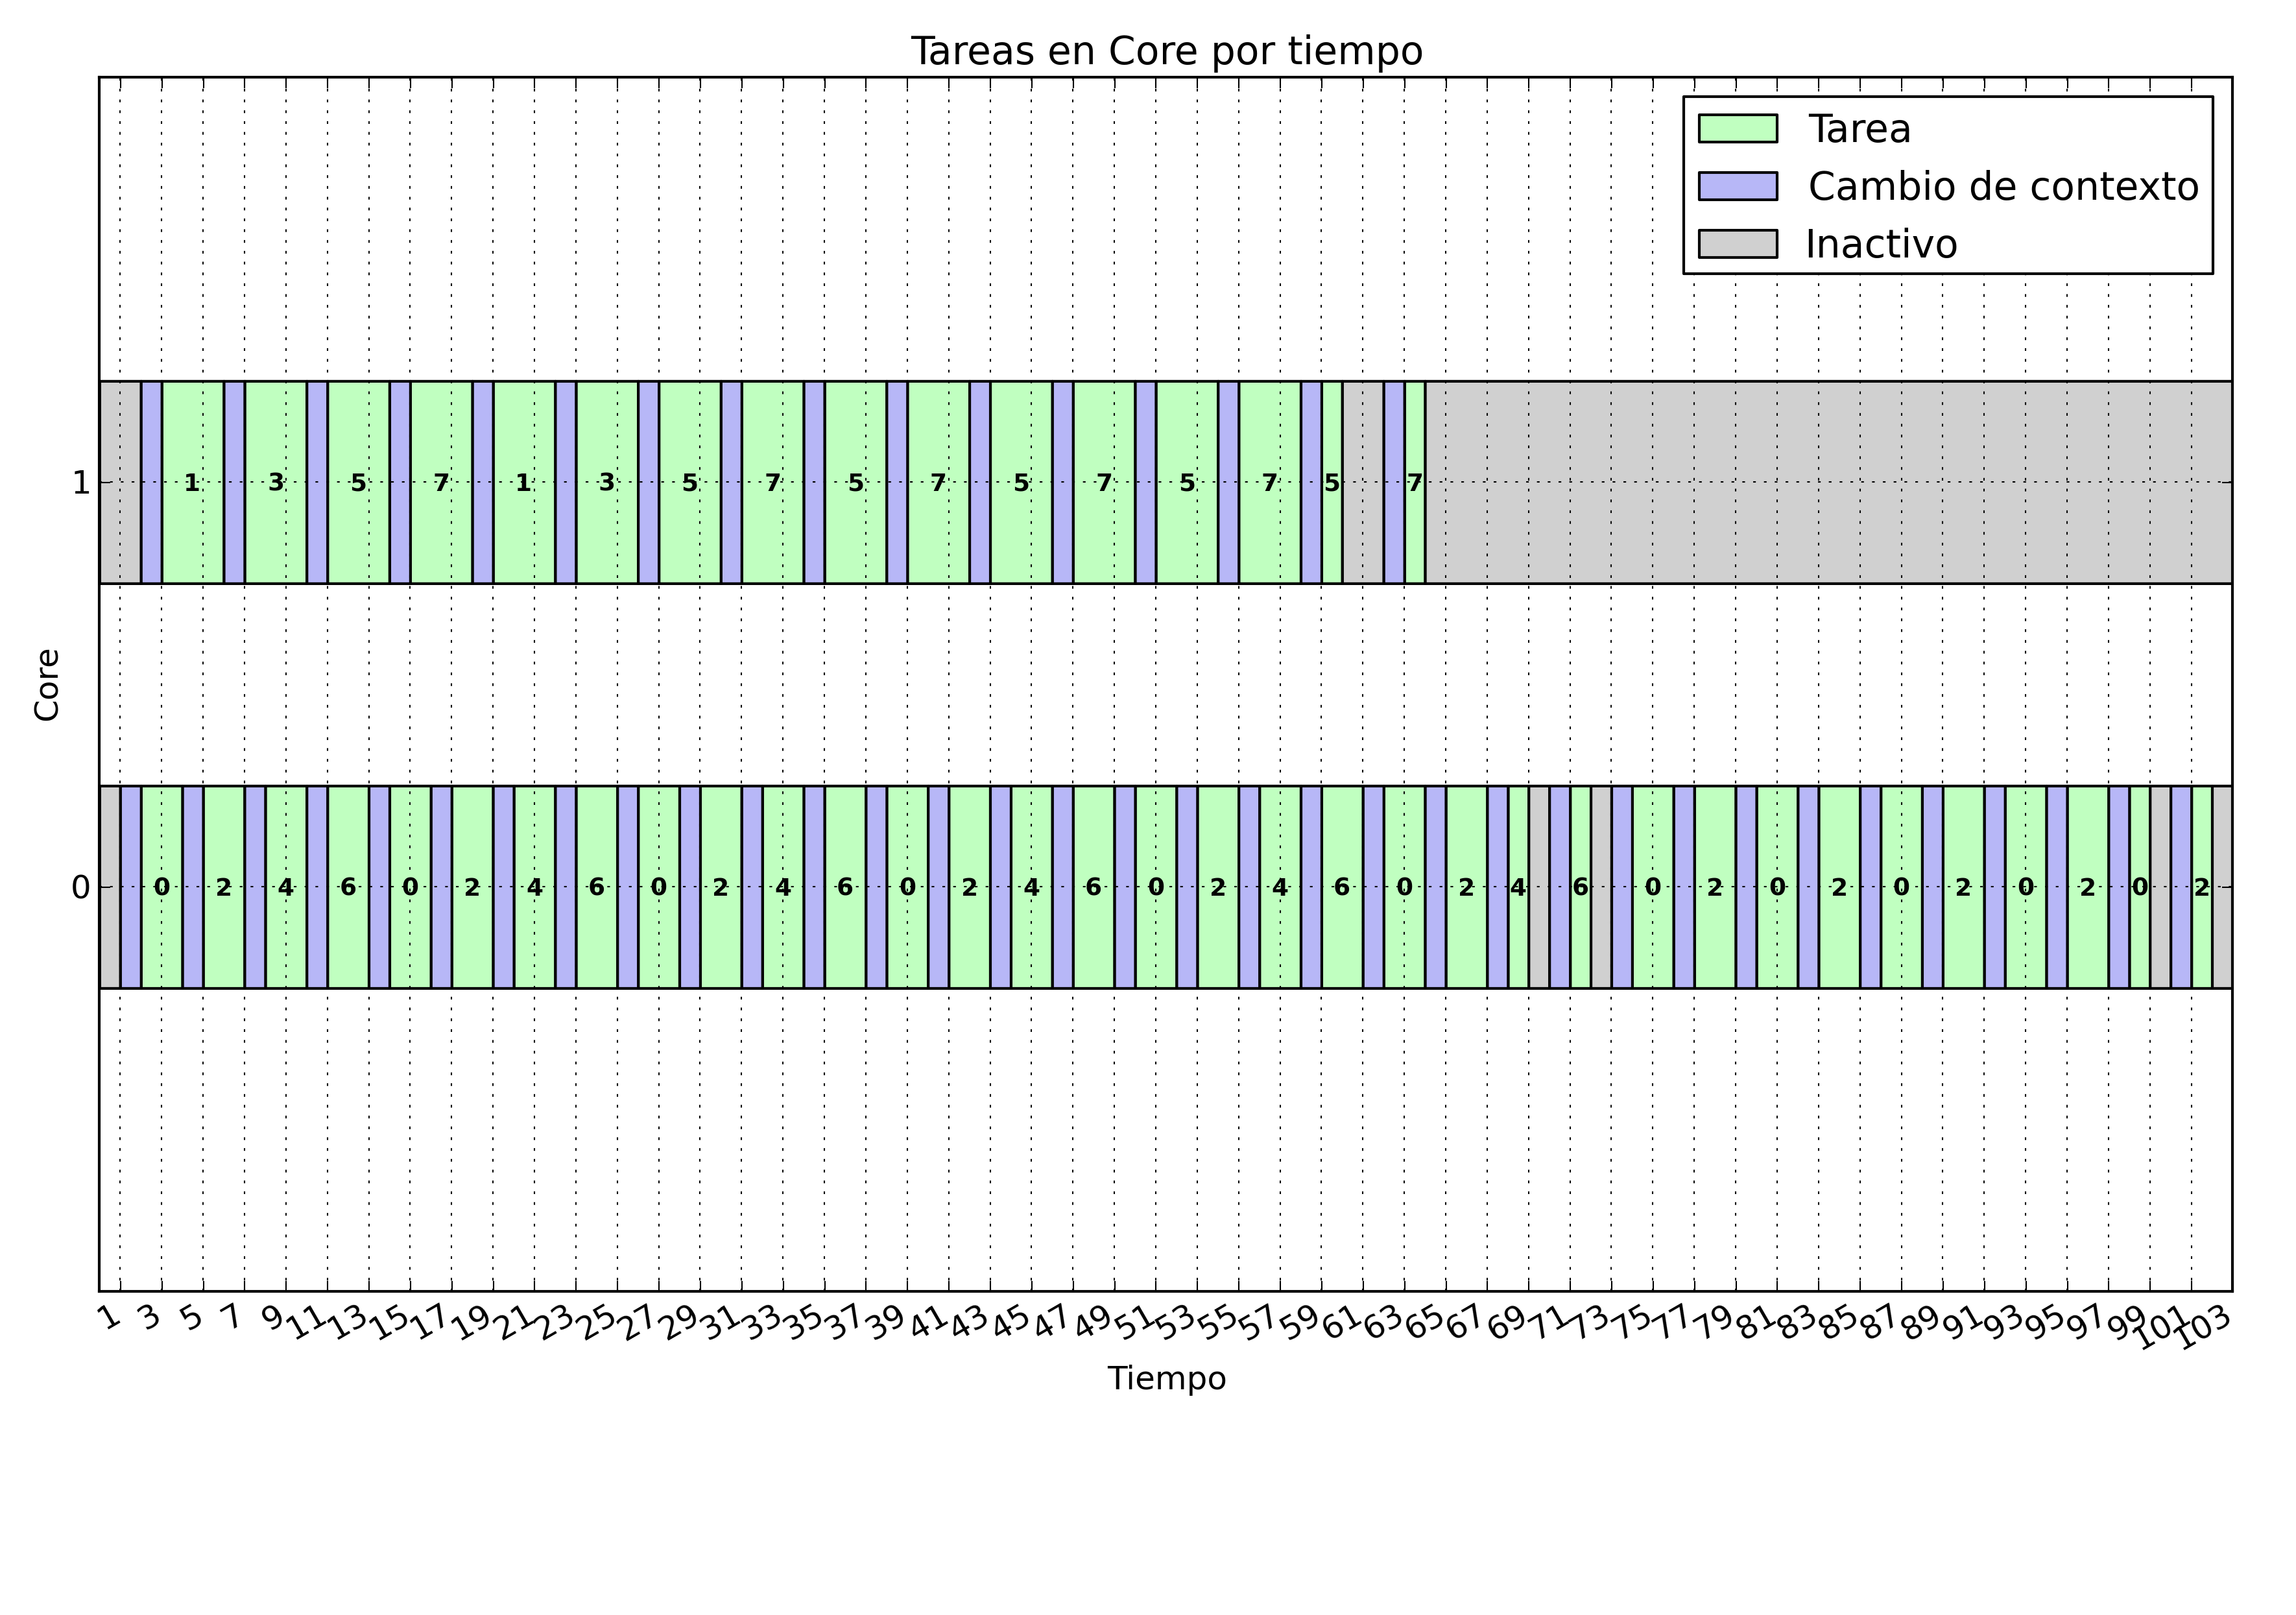
\includegraphics[width=\textwidth]{ej8/figs/C2Q3sinMigracion.png}
  \caption{Diagramas de procesadores sin migración.}
\end{figure}

Como se ve en los gráficos, el resultado confirma la hipótesis propuesta. Efectivamente, la reducción en el tiempo de ejecución fue mayor en el caso del scheduler con migración.

Por último, consideramos que variar el costo de migración entre los núcleos, solo podría extender el tiempo de ejecución en el scheduler con migración. Dado que no causa ningun otro efecto relevante en comparación, no se realizó experimentación de este caso.




% -------------------------------------------------------
% Ejercicio 9
% -------------------------------------------------------
\section{Ejercicio 9}

El objetivo en esta sección es romper el algoritmo de probabilidades fijas pero no el de dinámicas. Presentamos el siguiente lote:

\begin{lstlisting}
# Tareas cortas y frecuentes
&A7,6,1
# Tareas largas y poco frecuentes
&B3,13,4
\end{lstlisting}

Intuitivamente, la idea es crear procesos que sean más o menos largos, y que tengan un período largo (para que tengan una prioridad fija baja).
Luego, hay que crear muchos procesos cortos que le saquen tiempo a los procesos largos. En nuestro lote la familia A es de procesos cortos y la B de procesos largos.

Los procesos de la familia A, en el scheduler de prioridad fija, van a sacarle la cpu siempre a los de la B.
Sin embargo, el scheduler de prioridad dinámica ``se da cuenta'' cuando la deadline de los procesos de familia B se acerca, y los prioriza cuando eso pasa.

\begin{figure}[h]
 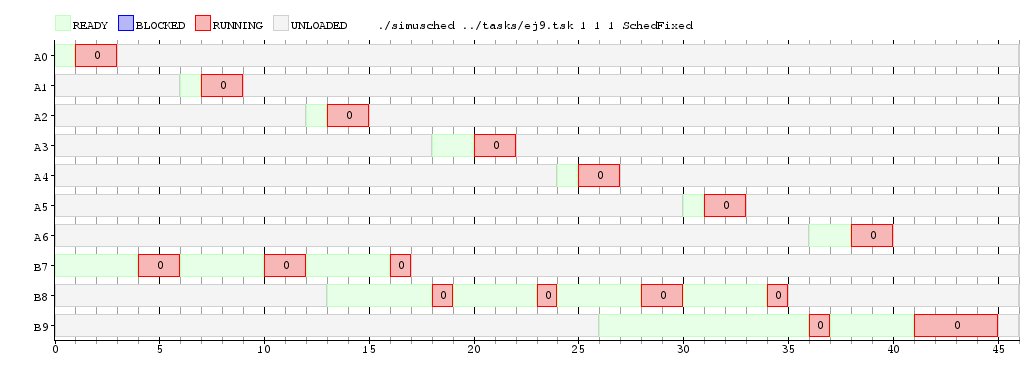
\includegraphics[width=\textwidth]{ej9/figs/fixed.png}
 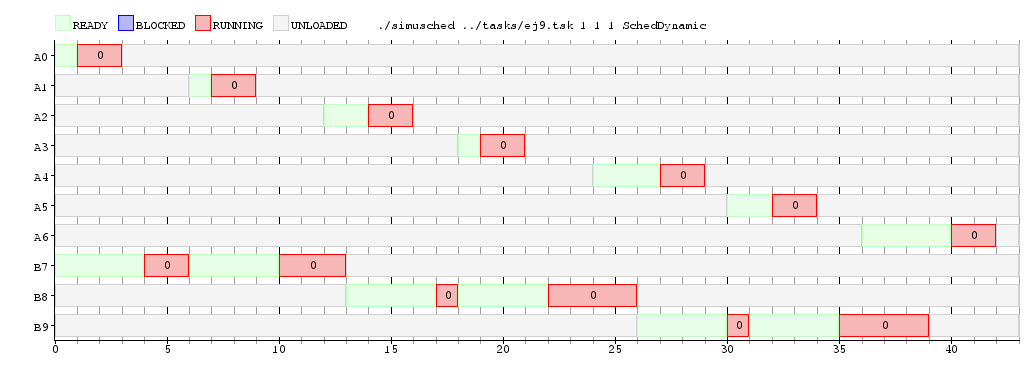
\includegraphics[width=\textwidth]{ej9/figs/dynamic.png}
 \caption{Diagramas de Gantt sobre el lote de tareas, para el algoritmo de prioridades fijas (arriba) y el de prioridades dinámicas (abajo).}
 \label{fig:ej9}
\end{figure}

Vemos en la figura~\ref{fig:ej9} que la deadline del proceso B7 no se cumple (tiene período 13 y se completa en el tick número 17).
En cambio en el algoritmo de prioridades dinámicas, se posterga la ejecución de A2 para poder cumplir la deadline de B7.
Esto no le impide terminar con el proceso A2 también.


% -------------------------------------------------------
% Ejercicio 10
% -------------------------------------------------------
\section{Ejercicio 10}


\newpage
\bibliographystyle{plain}
\bibliography{tp3}

\end{document}

